Пусть есть некоторая тяжелая нить, т.е. кривая AB, обладающая массой.
Пусть кривая спрямляемая и нам известна масса любого кусочка кривой AB.
Т.е. если возьмем точку $M \in AB$, тогда:

\begin{wrapfigure}{r}[5pt]{0.4\textwidth}
\centering 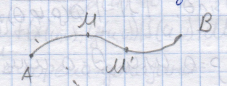
\includegraphics[scale=1]{im.png}
\end{wrapfigure}

Если нить однородна, т.е массы кусочков кривой одинаковой длинны равны,
по отношению массы нити к длине, т.е масса нити единичной длинны называется плотностью

Если нить не однородна, то назовем средней плотностью участка MM' отношение массы участка MM' к
длине MM' $(\frac{\triangle m}{\triangle l})$.
Если $\exists(\lim\limits_{\triangle l \rightarrow 0}\frac{\triangle m}{\triangle l} = A)[A \rightarrow \inf]$, то величина A - это плотность нити в точке $M (\varrho (M) )$.

Пусть известнна плотность нити в каждой точке $(\varrho (M) )$ и нужно определить ее массу.
Для этого разобъем кривую AB точками ${A_i}_{i=0}^{n}\max$,
что $A_0 = A, A_n = B$, причем плотность на отрезке $[A_{i-1}; A_i]$ равна плотности
в $A_i(\varrho ([A_{i-1}; A_i] = \varrho (A_i))$.
Тогда масса дуги $A_{i-1}A_i \approx \varrho (A_i)\triangle l_i ,
где \triangle l_i = \triangle l_i = l_{\overset {\smile} {A_{i-1}{A_i}}}$.

Тогда масса всей нити $AB \approx \sum_{i=1}^{n} \varrho (A_i)\triangle l_i$, и ясно,
что чем меньше разбиение, тем меньше ошибка (и значение суммы будет более близким к массе нити).
Если возьмем $\alpha = \max\limits_{1 \lq i \lq n}\triangle l_i$, то за массу нити возьмем $\lim\limits_{\alpha \rightarrow 0} \sum_{i=1}^{n} \varrho (A_i)\triangle l_i$.

Масса нити не зависит от того, какую точку взять начальной, а длина не зависит от концов.



